\left( % !TeX program = xelatex 
\documentclass{hitreport}
\usepackage{url}
\usepackage{algorithm,float}  
\usepackage{algpseudocode}  
\usepackage{amsmath}
\usepackage{cite}
\usepackage{threeparttable}
\usepackage{subfig}
\usepackage{listings} %插入代码
\usepackage{xcolor} %代码高亮
\usepackage{tikz}
\usepackage{hyperref}



\lstset{numbers=left, %设置行号位置
	numberstyle=\tiny, %设置行号大小
	keywordstyle=\color{blue}, %设置关键字颜色
	commentstyle=\color[cmyk]{1,0,1,0}, %设置注释颜色
	frame=single, %设置边框格式
	escapeinside=``, %逃逸字符(1左面的键),用于显示中文
	breaklines, %自动折行
	extendedchars=false, %解决代码跨页时,章节标题,页眉等汉字不显示的问题
	xleftmargin=2em,xrightmargin=2em, aboveskip=1em, %设置边距
	tabsize=4, %设置tab空格数
	showspaces=false %不显示空格
}

\renewcommand{\algorithmicrequire}{\textbf{Input:}}  % Use Input in the format of Algorithm  
\renewcommand{\algorithmicensure}{\textbf{Output:}} % Use Output in the format of Algorithm  

\makeatletter
\newenvironment{breakablealgorithm}
  {% \begin{breakablealgorithm}
   \begin{center}
     \refstepcounter{algorithm}% New algorithm
     \hrule height.8pt depth0pt \kern2pt% \@fs@pre for \@fs@ruled
     \renewcommand{\caption}[2][\relax]{% Make a new \caption
       {\raggedright\textbf{\ALG@name~\thealgorithm} ##2\par}%
       \ifx\relax##1\relax % #1 is \relax
         \addcontentsline{loa}{algorithm}{\protect\numberline{\thealgorithm}##2}%
       \else % #1 is not \relax
         \addcontentsline{loa}{algorithm}{\protect\numberline{\thealgorithm}##1}%
       \fi
       \kern2pt\hrule\kern2pt
     }
  }{% \end{breakablealgorithm}
     \kern2pt\hrule\relax% \@fs@post for \@fs@ruled
   \end{center}
  }
\makeatother

% =============================================
% Part 0 Edit the info
% =============================================

\major{计算机科学与技术}
\name{孙骁}
\title{机器学习实验报告}
\stuid{1180300811} % 学号
\college{计算学部}
\date{2020年11月3日}
\lab{} %实验地点
\course{机器学习}
\instructor{刘扬}
% \grades{}
\expname{GMM模型} %实验名称
% \exptype{} % 实验类型
% \partner{} % 同组学生名字
\term{2020秋季学期}

\begin{document}

\maketitle

\tableofcontents
\newpage
% =============================================
% Part 1 Header
% =============================================



% =============================================
% Part 2 Main document
% =============================================

\section{实验目的和要求}

\subsection{实验题目}
实现k-means聚类方法和混合高斯模型.

\subsection{实验目标}
实现一个k-means算法和混合高斯模型,并且用EM算法估计模型中的参数.

\subsection{实验测试}

用高斯分布产生\textit{k}个高斯分布的数据(不同均值和方差)(其中参数自己设定).
\begin{enumerate}
\item 用k-means聚类,测试效果;
\item 用混合高斯模型和你实现的EM算法估计参数,看看每次迭代后似然值变化情况,考察EM算法是否可以获得正确的结果(与你设定的结果比较).
\end{enumerate}

\subsection{实验应用}
可以UCI上找一个简单问题数据,用你实现的GMM进行聚类.

\section{实验环境}

\begin{enumerate}
\item Anaconda 4.8.4
\item Python 3.7.4
\item PyCharm 2019.1 (Professional Edition)
\item Windows 10 2004
\end{enumerate}

\section{实验原理}

\subsection{聚类问题}

聚类问题属于无监督学习问题. 假定样本集$D = \left\{\boldsymbol{x}_1, \boldsymbol{x}_2, \cdots, \boldsymbol{x}_m\right\}$包含\textit{m}个无标记样本,每个样本 $\boldsymbol{x}_i=\left(x_{i1} ; x_{i2} ; \cdots ; x_{in}\right)$是一个\textit{n}维特征向量,则聚类算法将样本集\textit{D}划分为\textit{k}个不相交的簇$\left\{C_l|l=1,2,\cdots, k\right\}$,其中$C_{l'}\cap_{l'\ne l}C_{l} = \varnothing$. 相应的,我们用$\lambda_j\in \left\{1,2, \cdots, k\right\}$表示样本$\boldsymbol{x}_j$的“簇标记”,即$\boldsymbol{x}_j\in C_{\lambda_j}$. 于是,聚类的结果可以用包含\textit{m}个元素的簇标记向量$\boldsymbol{\lambda} = \left(\lambda_1;\lambda_2;\cdots;\lambda_m\right)$表示.

\subsection{K-Means算法原理}

对于给定的样本集$D = \left\{\boldsymbol{x}_1, \boldsymbol{x}_2, \cdots, \boldsymbol{x}_m\right\}$, “\textit{k}均值”算法针对聚类所得到的簇划分$\mathcal{C} = \left\{C_1, C_2, \cdots, C_k\right\}$最小化平方误差
\begin{align}\label{equ:E}
E = \sum_{i=1}^{k}\sum_{\boldsymbol{x}\in C_i}{\lVert \boldsymbol{x} -\boldsymbol{\mu_i} \rVert}_{2}^{2},
\end{align}
其中$\boldsymbol{\mu_i} = \frac{1}{\lvert C_i \rvert}\sum_{\boldsymbol{x} \in C_i} \boldsymbol{x}$是簇$C_i$的均值向量. 式(\ref{equ:E})刻画了簇内样本围绕均值向量的紧密程度,\textit{E}值越小,则簇内样本相似度越高. 

最优化式(\ref{equ:E})并不容易,找到其最优解需要考查样本集\textit{D}所有可能的簇划分,显然这是一个NP难问题. 因此,\textit{k}均值算法采用了贪心策略,通过迭代优化来近似最小化式(\ref{equ:E}). 



\subsection{混合高斯模型}

对于\textit{n}维样本空间$\mathcal{X}$中的随机变量$\boldsymbol{x}$,若$\boldsymbol{x}$服从高斯分布,其概率密度函数为
\begin{align}\label{equ:gauss}
p\left(\boldsymbol{x}\right) = \dfrac{1}{\left(2\pi\right)^{\frac{n}{2}} \lvert \boldsymbol{\Sigma} \rvert^{\frac{1}{2}}} \exp \left(-\dfrac{1}{2} \left(\boldsymbol{x}-\boldsymbol{\mu}\right)^{\text{T}} \boldsymbol{\Sigma}^{-1} \left(\boldsymbol{x} - \boldsymbol{\mu}\right)\right),
\end{align}
其中$\boldsymbol{\mu}$是\textit{n}维均值向量,$\boldsymbol{\Sigma}$是$n\times n$的协方差矩阵,由式(\ref{equ:gauss})可知,高斯分布完全由均值向量$\boldsymbol{\mu}$和协方差矩阵$\boldsymbol{\Sigma}$这两个参数决定,因此我们也将概率密度函数记为$p\left(\boldsymbol{x} | \boldsymbol{\mu}, \boldsymbol{\Sigma}\right)$.

\begin{definition}[混合高斯分布]
定义高斯混合分布如下:
\begin{align}\label{equ:hmm}
p_{\mathcal{M}}\left(\boldsymbol{x}\right) = \sum\limits_{i=1}^k{\alpha_i\cdot p\left(\boldsymbol{x} | \boldsymbol{\mu}_i, \boldsymbol{\Sigma}_i\right)},
\end{align}
该分部共由\textit{k}个混合成分组成,每个混合成分对应一个高斯分布. 其中$\boldsymbol{\mu}_i$与$\boldsymbol{\Sigma}_i$是第\textit{i}个高斯混合成分的参数,而$\alpha_i>0$为相应的“混合系数”,且$\sum_{i=1}^{k}\alpha_i = 1$.
\end{definition}

假设样本的生成过程由高斯混合分布给出:首先,根据$\alpha_1, \alpha_2, \cdots, \alpha_k$定义的先验分布选择高斯混合成分,即$p\left(z_j = i\right) = \alpha_i$,其中$\alpha_i$是选择第\textit{i}个混合成分的概率;然后,根据被选择的混合成分的概率密度进行采样,从而生成相应的样本. 根据贝叶斯定理,$z_j$的后验分布如式(\ref{equ:pmzx})所示,
\begin{align}\label{equ:pmzx}
\begin{split}
p_{\mathcal{M}}\left(z_j = i|\boldsymbol{x}_j\right) & = \frac{P\left(z_j=i\right)\cdot p_{\mathcal{M}}\left(\boldsymbol{x}_j|z_j = i\right)}{p_{\mathcal{M}}\left(\boldsymbol{x}_j\right)}\\
& = \frac{\alpha_i\cdot p\left(\boldsymbol{x}_j|\boldsymbol{\mu}_i, \boldsymbol{\Sigma}_i\right)}{\sum\limits_{l=1}^{k}\alpha_l\cdot p\left(\boldsymbol{x}_j|\boldsymbol{\mu}_l, \boldsymbol{\Sigma}_l\right)},
\end{split}
\end{align}
即$p_{\mathcal{M}}\left(z_j = i|\boldsymbol{x}_j\right)$给出了样本$\boldsymbol{x}_j$由第\textit{i}个高斯混合成分生成的后验概率.

当混合高斯分布(\ref{equ:hmm})已知时,混合高斯聚类算法将把样本集\textit{D}划分为\textit{k}个簇$\mathcal{C} = \left\{C_1,C_2, \cdots, C_k\right\}$,每个样本$\boldsymbol{x}_j$的簇标记$\lambda_j$如式(\ref{equ:classif})确定:
\begin{align}\label{equ:classif}
\lambda_j = \underset{i\in \left\{1,2,\cdots,k\right\}}{\arg\max}\gamma_{ji}.
\end{align}

对于给定样本集\textit{D}式(\ref{equ:hmm})中的模型参数$\left\{\left(\alpha_i, \boldsymbol{\mu}_i, \boldsymbol{\Sigma}_i\right)|1\le i\le k\right\}$的求解,可以采用极大似然估计,即最大化对数似然
\begin{align}\label{equ:lld}
\begin{split}
LL\left(D\right) & = \ln \left(\prod_{j=1}^{m}p_{\mathcal{M}}\left(\boldsymbol{x}_j\right)\right)\\
& = \sum_{j=1}^{m}\ln \left(\sum_{i=1}^{k}\alpha_i\cdot p\left(\boldsymbol{x}_j| \boldsymbol{\mu}_i, \boldsymbol{\Sigma}_i\right)\right),
\end{split}
\end{align}

对于以上问题的最优化求解,常采用EM算法进行迭代优化. 

\subsection{EM算法}

若参数$\left\{\left(\alpha_i, \boldsymbol{\mu}_i, \boldsymbol{\Sigma}_i\right)|1\le i\le k\right\}$能使得式(\ref{equ:lld})最大化,则由$\frac{\partial LL\left(D\right)}{\partial\boldsymbol{\mu}_i} = 0$有
\begin{align}
\sum\limits_{j=1}^{m}\frac{\alpha_i\cdot p\left(\boldsymbol{x}_j|\boldsymbol{\mu}_i,\boldsymbol{\Sigma}_i\right)}{\sum\limits_{l=1}^{k}\alpha_l\cdot p\left(\boldsymbol{x}_j|\boldsymbol{\mu}_l,\boldsymbol{\Sigma}_l\right)}\left(\boldsymbol{x}_j-\boldsymbol{\mu}_i\right) = 0,
\end{align}
由式(\ref{equ:pmzx})及$\gamma_{ji} = p_{\mathcal{M}}\left(z_j = i|\boldsymbol{x}_j\right)$,有
\begin{align}
\boldsymbol{\mu}_i = \frac{\sum\limits_{j=1}^{m}\gamma_{ji}\boldsymbol{x}_j}{\sum\limits_{j=1}^{m}\gamma_{ji}},
\end{align}
即各混合成分的均值可以通过样本加权平均来估计,样本权重是每个样本属于该成分的后验概率. 类似的,由$\frac{\partial LL\left(D\right)}{\partial \boldsymbol{\Sigma}_i} = 0$可得
\begin{align}
\boldsymbol{\Sigma}_i = \frac{\sum\limits_{j=1}^{m}\gamma_{ji}\left(\boldsymbol{x}_j-\boldsymbol{\mu}_i\right)\left(\boldsymbol{x}_j - \boldsymbol{\mu}_i\right)^{\text{T}}}{\sum\limits_{j=1}^{m}\gamma_{ji}},
\end{align}
对于混合系数$\alpha_i$,除了要最大化$LL\left(D\right)$,还需要满足$\alpha_i\ge 0$,$\sum_{i=1}^{k}\alpha_i=1$,考虑$LL\left(D\right)$的拉格朗日形式
\begin{align}\label{equ:lldlam}
LL\left(D\right) + \lambda\left(\sum_{i=1}^{k}\alpha_i-1\right),
\end{align}
其中$\lambda$为拉格朗日乘子. 由式(\ref{equ:lldlam})对$\alpha_i$的导数为0,有
\begin{align}
\sum\limits_{j=1}^{m}\frac{\alpha_i\cdot p\left(\boldsymbol{x}_j|\boldsymbol{\mu}_i,\boldsymbol{\Sigma}_i\right)}{\sum\limits_{l=1}^{k}\alpha_l\cdot p\left(\boldsymbol{x}_j|\boldsymbol{\mu}_l,\boldsymbol{\Sigma}_l\right)}+\lambda = 0.
\end{align}
两边同时乘以$\alpha_i$,对所有样本求和可知$\lambda = -m$,有
\begin{align}
\alpha_i = \frac{1}{m}\sum_{j=1}^{m}\gamma_{ji},
\end{align}
即每个高斯成分的混合系数由样本属于该成分的平均后验概率确定. 



\section{算法实现}
\subsection{K-Means算法}\label{sec:kmeans}

K-Means算法的迭代优化算法如算法(\ref{alg:kmeans})所示.

\begin{breakablealgorithm}
  \caption{ K Means}  
  \label{alg:kmeans}  
  \begin{algorithmic}[1] 
    \Require  
    $D = \left\{\boldsymbol{x}_1, \boldsymbol{x}_2, \cdots, \boldsymbol{x}_m\right\}$, 聚类簇数\textit{k}
    \Ensure  
   	簇划分$\mathcal{C} = \left\{C_1, C_2, \cdots, C_k\right\}$
   	\State 从\textit{D}中随机选择\textit{k}个样本作为初始均值向量$\left\{\boldsymbol{\mu_1}, \boldsymbol{\mu_2}, \cdots, \boldsymbol{\mu_k}\right\}$
   	\Repeat
   		\State 令$C_i = \varnothing \left(1\le i\le k\right)$
   		\For{$j=1,2\cdots, m$}
   		\State 计算样本$\boldsymbol{x}_j$与各均值向量$\boldsymbol{\mu_i}\left(1\le i\le k\right)$的距离:$d_{ji} = \lVert \boldsymbol{x}_j - \boldsymbol{x}_i \rVert_{2}$;
   		\State 根据距离最近的均值向量确定$\boldsymbol{x}_j$的簇标记:$\lambda_j = \arg \min_{i\in \left\{1,2,\cdots, k\right\}} d_{ji}$;
   		\State 将样本$\boldsymbol{x}_j$划入相应的簇:$C_{\lambda_j} = C_{\lambda_j}\cup \left\{\boldsymbol{x}_j\right\}$;
   		\EndFor
   		\For{$i=1,2,\cdots, k$}
   		\State 计算新均值向量:$\boldsymbol{\mu_i'} = \frac{1}{\lvert C_i \rvert}\sum_{\boldsymbol{x} \in C_i} \boldsymbol{x}$;
   		\If{$ \boldsymbol{\mu_i'} \ne \boldsymbol{\mu_i}$}
   		\State 将当前均值向量$\boldsymbol{\mu_i}$更新为$\boldsymbol{\mu_i'}$
   		\Else
   		\State 保持当前均值向量不变
   		\EndIf
   		\EndFor
   	\Until{当前均值向量均未更新}
  \end{algorithmic}  
\end{breakablealgorithm}



\subsection{高斯混合聚类算法}\label{sec:gauss}

高斯混合聚类算法描述如算法(\ref{alg:gauss})所示,算法首先对高斯混合分布的模型参数进行了初始化. 然后在第2-12行基于EM算法对模型参数进行迭代更新. 若EM算法的停止条件满足(最大迭代轮数,或似然函数$LL\left(D\right)$增长很少甚至不再增长),则在第14-17行根据高斯混合分布确定簇划分,并最后返回最终结果.



\begin{breakablealgorithm}
  \caption{Gaussian mixture clustering algorithm}  
  \label{alg:gauss}  
  \begin{algorithmic}[1] 
    \Require  
    $D = \left\{\boldsymbol{x}_1, \boldsymbol{x}_2, \cdots, \boldsymbol{x}_m\right\}$, 高斯混合成分个数\textit{k}
    \Ensure  
   	簇划分$\mathcal{C} = \left\{C_1, C_2, \cdots, C_k\right\}$
   	\State 初始化高斯混合分布的模型参数$\left\{\left(\alpha_i, \boldsymbol{\mu}_i, \boldsymbol{\Sigma}_i\right)|1\le i\le k\right\}$
   	\Repeat
   		\For{$j=1,2,\cdots, m$}
   		\State 根据式(\ref{equ:pmzx})计算计算 $\gamma_{ji} = p_{\mathcal{M}}\left(z_j = i|\boldsymbol{x}_j\right) \left(1\le i\le k\right)$
   		
   		\EndFor
   		\For{$i=1,2,\cdots,k$}
   		\State 计算新均值向量:$\boldsymbol{\mu'}_i = \frac{\sum_{j=1}^{m}\gamma_{ji}\boldsymbol{x}_j}{\sum_{j=1}^{m}\gamma_{ji}}$;
   		\State 计算新协方差矩阵:$\boldsymbol{\Sigma'}_i = \frac{\sum_{j=1}^{m}\gamma_{ji}\left(\boldsymbol{x}_j-\boldsymbol{\mu'}_i\right)\left(\boldsymbol{x}_j - \boldsymbol{\mu'}_i\right)^{\text{T}}}{\sum_{j=1}^{m}\gamma_{ji}}$;
   		\State 计算新混合系数:$\alpha_i' = \frac{\sum_{j=1}^{m}\gamma_{ji}}{m}$;
   		\EndFor
   		\State 将模型参数$\left\{\left(\alpha_i, \boldsymbol{\mu}_i, \boldsymbol{\Sigma}_i\right)|1\le i\le k\right\}$更新为$\left\{\left(\alpha_i', \boldsymbol{\mu'}_i, \boldsymbol{\Sigma'}_i\right)|1\le i\le k\right\}$
   	\Until{满足停止条件}
   	\State $C_i = \varnothing \left(1\le i\le k\right)$
   	\For{$j=1,2,\cdots,m$}
   	\State 根据式(\ref{equ:classif})确定$\boldsymbol{x}_j$的簇标记$\lambda_j$;
   	\State 将$\boldsymbol{x}_j$划入相应的簇:$C_{\lambda_j} = C_{\lambda_j}\cup \left\{\boldsymbol{x}_j\right\}$
   	\EndFor
  \end{algorithmic}  
\end{breakablealgorithm}





\section{实验步骤}

\subsection{生成满足二维高斯分布数据}

依照给定的均值和方差,生成指定数量的满足二维高斯分布的数据,生成三类数据,二维均值分别为1、1;-1、0;1、-2,二维协方差矩阵为$\left( \begin{matrix}
	0.1&		0\\
	0&		0.1\\
\end{matrix} \right) $,生成三类数据各生成100个. 

%\lstinputlisting[language=python]{code/PolynomialFitting.py}

\subsection{实现章节\ref{sec:kmeans}中的K\_Means算法}

实现实现章节\ref{sec:kmeans}中的K-Means算法,代码见附录(\ref{app:kmeans}).

\subsection{实现章节\ref{sec:gauss}中的混合高斯模型}

实现章节\ref{sec:gauss}中的混合高斯模型,并使用EM算法进行求解,代码见附录(\ref{app:gmm}).

\subsection{使用UCI数据集测试K-Means与混合高斯模型}
选用UCI鸢尾花分类数据集,根据鸢尾花的4个属性对鸢尾花的分类进行预测. 数据集中一共有三种类别,每个类别各50个样本,一共150个样本,每条数据包括四个特征,分别是:
\begin{enumerate}
\item 萼片长度(单位:厘米)
\item 萼片宽度(单位:厘米)
\item 花瓣长度(单位:厘米)
\item 花瓣宽度(单位:厘米)
\end{enumerate}

实现章节\ref{sec:kmeans}中的K-Means算法与章节\ref{sec:gauss}中的混合高斯模型,并显示分类的准确率. 代码见附录(\ref{app:data}). 

\section{实验结果}

\subsection{K-Means聚类结果}

首先采用随机选取初始簇中心的方法,实验结果如图(\ref{fig:fig1})所示. 很明显在分类上出现了错误,分析原因为没有选好的选取初始簇中心,导致了聚类时无法区分与簇中心较远而距离大致相近的点.

\begin{figure}[htb]
	\centering
		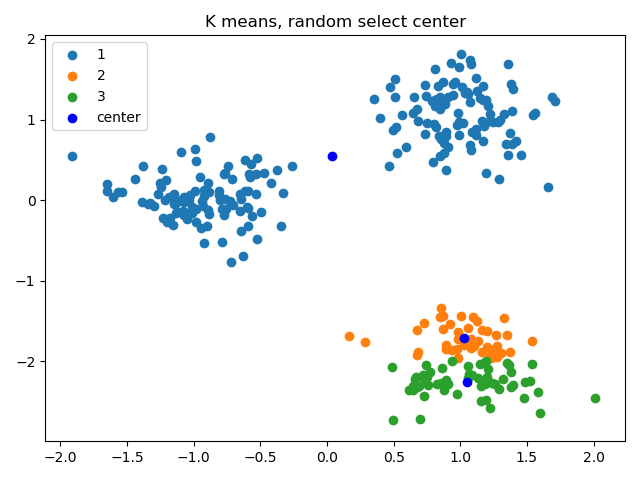
\includegraphics[width=.7\textwidth]{kmeansrandom.png}
	\caption{随机选取初始簇中心的K-Means算法结果}\label{fig:fig1}
\end{figure}

第二次选择了选择相距尽可能远的点作为初始的簇中心,聚类结果如图(\ref{fig:fig2})所示,此次初始簇中心相距较远,较好的划分了样本集.

\begin{figure}[htb]
	\centering
		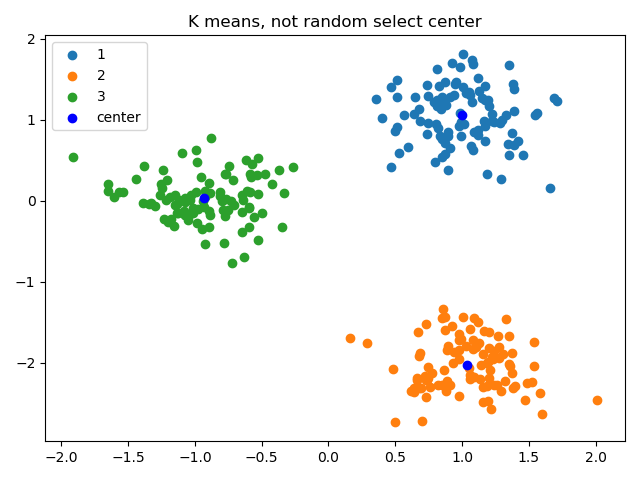
\includegraphics[width=.7\textwidth]{kmeansnotrandom.png}
	\caption{非随机选取初始簇中心的K-Means算法结果}\label{fig:fig2}
\end{figure}

\subsection{混合高斯模型聚类结果}

混合高斯模型的聚类结果如图(\ref{fig:fig3}),可以看出和K-Means聚类效果基本一致.

\begin{figure}[htb]
	\centering
		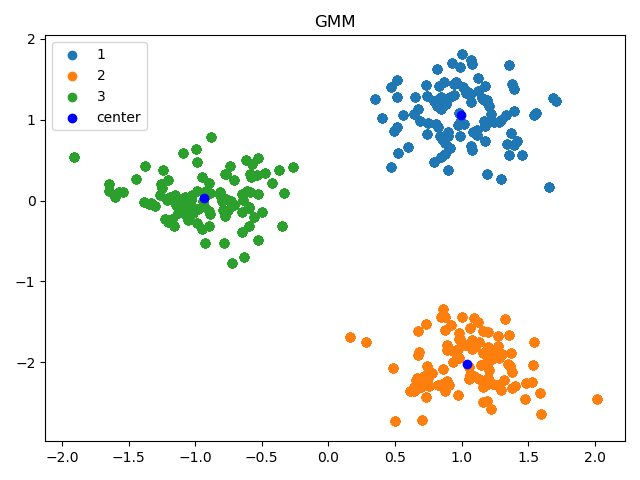
\includegraphics[width=.7\textwidth]{gmm.png}
	\caption{混合高斯模型的聚类结果}\label{fig:fig3}
\end{figure}

\subsection{使用UCI数据集测试K-Means与混合高斯模型}

数据集没有数据特征缺失的情况,对数据集分别使用K-Means算法聚类与基于EM算法的高斯混合模型聚类,得到的结果如图(\ref{fig:fig4})所示. 

\begin{figure}
	\centering
	
\includegraphics[width=0.7\linewidth]{iris.jpeg}
	\caption{在UCI鸢尾花数据集上测试结果}\label{fig:fig4}
\end{figure}



\section{实验结论}

\begin{enumerate}
\item K-Means聚类假设数据分布在以簇中心为中心的一定范围内,混合高斯模型则假设数据符合混合高斯分布;
\item 由于K-Means聚类算法采用贪心的思想,未必能得到全局最优解,簇中心初始化对于最终的结果有很大的影响,如果选择不好初始的簇中心值容易使之陷入局部最优解;
\item 使用EM算法解决混合高斯模型聚类问题时,如果初始高斯模型的均值和方差选取不当,可能会出现极大似然值为0的情况,也会出现协方差矩阵不可逆的情况.
\end{enumerate}

\renewcommand\refname{参考文献}
 
\begin{thebibliography}{2}
\bibitem{book:li}
李航, 统计学习方法(2019.3).

\bibitem{book:zhou}
周志华, 机器学习(2016.1).

\bibitem{url:bank}
\href{http://archive.ics.uci.edu/ml/datasets/Iris}{Iris Data Set. (1988.7) [Data set]}.
\end{thebibliography}

\newpage
\begin{appendices}

\section{K-Means算法--k\_means.py}\label{app:kmeans}
\begin{lstlisting}[language=python]
import numpy as np
import random
import collections


def calculate_distance(x_1, x_2):
    return np.linalg.norm(x_1 - x_2)


class KMeans(object):
    def __init__(self, data, k, deviation=1e-6):
        self.data = data
        self.k = k
        self.deviation = deviation
        self.data_rows = data.shape[0]
        self.data_columns = data.shape[1]
        self.data_attribution = [-1] * self.data_rows
        self.mu = self.__initial_k_dots()

    def __initial_k_dots(self):
        mu_temp = np.random.randint(0, self.k) + 1
        mu = [self.data[mu_temp]]
        for i in range(self.k - 1):
            ans = []
            for j in range(self.data_rows):
                temp_ans = np.sum([calculate_distance(self.data[j], mu[k]) for k in range(len(mu))])
                ans.append(temp_ans)
            mu.append(self.data[np.argmax(ans)])
        return np.array(mu)

    def k_means(self):
        number = 0
        while True:
            result = collections.defaultdict(list)
            for i in range(self.data_rows):
                distance = [calculate_distance(self.data[i], self.mu[j]) for j in range(self.k)]
                lam_j = np.argmin(distance)
                result[lam_j].append(self.data[i].tolist())
                self.data_attribution[i] = lam_j
            new_mu = np.array([np.mean(result[i], axis=0).tolist() for i in range(self.k)])
            new_loss = np.sum(calculate_distance(self.mu[i], new_mu[i]) for i in range(self.k))
            if new_loss > self.deviation:
                self.mu = new_mu
            else:
                break
            # print(number)
            number += 1
        # print(self.mu)
        return self.mu, result

    def random_select_center(self):
        self.mu = self.data[random.sample(range(self.data_rows), self.k)]
        return self.k_means()

    def not_random_select_center(self):
        self.mu = self.__initial_k_dots()
        return self.k_means()

\end{lstlisting}

\section{混合高斯模型与EM算法求解--gaussian\_mixture\_model.py}\label{app:gmm}
\begin{lstlisting}[language=python]
import numpy as np
import numpy.random as random
import collections
from scipy.stats import multivariate_normal


def calculate_distance(x_1, x_2):
    return np.linalg.norm(x_1 - x_2)


class GaussianMixtureModel(object):
    def __init__(self, data, k, deviation, iteration_number):
        self.data = data
        self.k = k
        self.deviation = deviation
        self.iteration_number = iteration_number
        self.alpha = np.ones(self.k) * (1.0 / self.k)
        self.data_rows = data.shape[0]
        self.data_columns = data.shape[1]
        self.mu, self.sigma = self.__init_params()
        self.data_attribution = [-1] * self.data_rows
        self.result = collections.defaultdict(list)
        self.gamma = None

    def __init_params(self):
        mu_0 = random.randint(0, self.k)
        # print(mu_0)
        mu_temp = [self.data[mu_0]]
        for index in range(self.k - 1):
            temp_ans = []
            for i in range(self.data_rows):
                temp_ans.append(np.sum([calculate_distance(self.data[i], mu_temp[j]) for j in range(len(mu_temp))]))
            mu_temp.append(self.data[np.argmax(temp_ans)])
        mu = np.array(mu_temp)
        # print("mu", mu)
        sigma = collections.defaultdict(list)
        for i in range(self.k):
            sigma[i] = np.eye(self.data_columns, dtype=float) * 0.1

        # print("sigma", sigma)
        # for i in range(self.k):
        #     print("sigma", i, sigma[i])
        return mu, sigma

    def calculate_likelihood(self):
        likelihood = np.zeros((self.data_rows, self.k))
        for i in range(self.k):
            # print("------------")
            # print("mu[i]", self.mu[i])
            # print("sigma[i]", self.sigma[i])
            likelihood[:, i] = multivariate_normal.pdf(self.data, self.mu[i], self.sigma[i])
            # print(likelihood[:, i])
        return likelihood

    def calculate_expectation(self):
        likelihoods = self.calculate_likelihood() * self.alpha
        sum_likelihood = np.expand_dims(np.sum(likelihoods, axis=1), axis=1)

        self.gamma = likelihoods / sum_likelihood
        # print(self.gamma)
        self.data_attribution = self.gamma.argmax(axis=1)
        for i in range(self.data_rows):
            self.result[self.data_attribution[i]].append(self.data[i].tolist())

    def max_function(self):
        for i in range(self.k):
            gamma_ji = np.expand_dims(self.gamma[:, i], axis=1)
            mu_i = (gamma_ji * self.data).sum(axis=0) / gamma_ji.sum()
            cov = (self.data - mu_i).T.dot((self.data - mu_i) * gamma_ji) / gamma_ji.sum()
            self.mu[i], self.sigma[i] = mu_i, cov
        self.alpha = self.gamma.sum(axis=0) / self.data_rows

    def gmm(self):
        pre_alpha = self.alpha
        pre_mu = self.mu
        pre_sigma = self.sigma
        for i in range(self.iteration_number):
            self.calculate_expectation()
            self.max_function()
            diff = np.linalg.norm(pre_alpha - self.alpha) + np.linalg.norm(pre_mu - self.mu) + np.sum(
                [np.linalg.norm(pre_sigma[i] - self.sigma[i]) for i in range(self.k)])
            if diff > self.deviation:
                pre_alpha = self.alpha
                pre_sigma = self.sigma
                pre_mu = self.mu
            else:
                break
        self.calculate_expectation()
        return self.mu, self.result

\end{lstlisting}

\section{读取鸢尾花数据集--read\_iris\_data.py}\label{app:data}
\begin{lstlisting}[language=python]
import numpy as np
import pandas as pd


def read_iris_data():
    data_set = pd.read_csv("../data/iris.csv")
    X = data_set.drop("class", axis=1)
    Y = data_set['class']
    # print(Y)
    return np.array(X, dtype=float), np.array(Y, dtype=str)

\end{lstlisting}

\section{主程序--k\_means\_GMM.py}\label{app:main}
\begin{lstlisting}[language=python]
import itertools as it

from matplotlib import pyplot as plt
from src.generate_data import *
from src.k_means import *
from src.read_iris_data import *
from src.gaussian_mixture_model import *


def generate_picture(k, random_mu, random_result, not_random_mu, not_random_result, gmm_mu, gmm_result):
    plt.title("K means, random select center")
    for i in range(k):
        plt.scatter(np.array(random_result[i])[:, 0], np.array(random_result[i])[:, 1], label=str(i + 1))
    plt.scatter(random_mu[:, 0], random_mu[:, 1], c="b", label="center")
    plt.legend()
    plt.show()

    plt.title("K means, not random select center")
    for i in range(k):
        plt.scatter(np.array(not_random_result[i])[:, 0], np.array(not_random_result[i])[:, 1], label=str(i + 1))
    plt.scatter(not_random_mu[:, 0], not_random_mu[:, 1], c="b", label="center")
    plt.legend()
    plt.show()

    plt.title("GMM")
    for i in range(k):
        plt.scatter(np.array(gmm_result[i])[:, 0], np.array(gmm_result[i])[:, 1], label=str(i + 1))
    plt.scatter(gmm_mu[:, 0], gmm_mu[:, 1], c="b", label="center")
    plt.legend()
    plt.show()


def test_iris_data():
    data_X, data_Y = read_iris_data()
    k_means = KMeans(data_X, 3)
    k_means__mu, k_means_result = k_means.not_random_select_center()
    k_means_attribution = k_means.data_attribution

    number = len(data_Y)
    counts_kmeans = []
    result = list(it.permutations(['Iris-setosa', 'Iris-versicolor', 'Iris-virginica'], 3))
    for i in range(len(result)):
        count = 0
        for index in range(number):
            # print(data_Y[index])
            # print(result[i][k_means_attribution[index]])
            if data_Y[index] == result[i][k_means_attribution[index]]:
                count += 1
        counts_kmeans.append(count)
    kmeans_accuracy = 1.0 * np.max(counts_kmeans) / number
    print("k means accuracy:", kmeans_accuracy)

    deviation = 1e-12
    iteration_number = 10000
    # print(data_X.shape)
    gmm = GaussianMixtureModel(data_X, 3, deviation, iteration_number)
    gmm_mu, gmm_result = gmm.gmm()

    counts_gmm = []
    gmm_attribution = gmm.data_attribution
    # print(gmm_attribution)
    for i in range(len(result)):
        count = 0
        for index in range(number):
            if data_Y[index] == result[i][gmm_attribution[index]]:
                count += 1
        counts_gmm.append(count)
    gmm_accuracy = 1.0 * np.max(counts_gmm) / number
    print("GMM accuracy:", gmm_accuracy)


def main():
    k = 3
    category_means = [[1, 1], [-1, 0], [1, -2]]
    category_number = [100, 100, 100]
    data = generate_2_dimension_data(category_means, category_number, k)
    k_means_result = KMeans(data, k)
    random_mu, random_result = k_means_result.random_select_center()
    not_random_mu, not_random_result = k_means_result.not_random_select_center()

    deviation = 1e-12
    iteration_number = 10000
    gmm = GaussianMixtureModel(data, k, deviation, iteration_number)
    gmm_mu, gmm_result = gmm.gmm()

    generate_picture(k, random_mu, random_result, not_random_mu, not_random_result, gmm_mu, gmm_result)

    test_iris_data()


if __name__ == '__main__':
    main()

\end{lstlisting}

\section{生成二维高斯分布数据--generate\_data.py}\label{app:gendata}
\begin{lstlisting}[language=python]
import numpy as np


def generate_2_dimension_data(category_means, category_number, k_number):
    cov = [[0.1, 0], [0, 0.1]]
    data = []
    for i in range(k_number):
        for index in range(category_number[i]):
            data.append(
                np.random.multivariate_normal([category_means[i][0], category_means[i][1]], cov).tolist())
    return np.array(data)

\end{lstlisting}

\end{appendices}

\end{document}
